\documentclass[12pt]{article}
\usepackage[margin=1in]{geometry} 
\usepackage{amsmath,amsthm,amssymb,amsfonts}
\usepackage{xspace}
\usepackage{graphicx}

\usepackage{titlesec}

\setcounter{secnumdepth}{4}
 
\newcommand{\N}{\mathbb{N}}
\newcommand{\Z}{\mathbb{Z}}
 
%\newenvironment{problem}[2][Problem]{\begin{trivlist}
%\item[\hskip \labelsep {\bfseries #1}\hskip \labelsep {\bfseries #2.}]}{\end{trivlist}}
%If you want to title your bold things something different just make another thing exactly like this but replace "problem" with the name of the thing you want, like theorem or lemma or whatever
 
\begin{document}
 
%\renewcommand{\qedsymbol}{\filledbox}
%Good resources for looking up how to do stuff:
%Binary operators: http://www.access2science.com/latex/Binary.html
%General help: http://en.wikibooks.org/wiki/LaTeX/Mathematics
%Or just google stuff

\newcommand{\newtext}[1]{\textcolor[rgb]{0.55,0.47,0.06}{#1}}

\newcommand{\mytext}[1]{{\normalfont{\textit{#1}}}}
\newcommand{\fifo}{FIFO\xspace}
\newcommand{\paritycheck}{Parity Check\xspace}
\newcommand{\vhdl}{VHDL\xspace}


\title{Pre-interview exercise: FIFO with Parity Check}
\author{Ariel Podlubne}
\maketitle
 
\section{Introduction}
The present report describes the work done to design and test a \fifo with a \paritycheck. The sections bellow describe all their parts and how they were designed.
 
\section{Design and Test}
The methodology for the design of the \fifo with the \paritycheck as well as for its test environment consisted in a layer design. This means that all the small internal modules were designed and tested first. Later, each one was incorporated into its corresponding ''outer''  layer or TOP module.  A description of each one and its simulation are shown below.

\subsection{\fifo and \paritycheck}
\label{sec:fifo and paritycheck}
This two modules were designed separately and each one tested with its own testbench.  Afterwards, they were both instantiated into a TOP module called \textit{FifoParityCheckerUB\_TOP}.

\subsubsection{\fifo}
\label{subsubsection: Fifo}
The \fifo has different input and output  ports, which can be divided in \textit{data}, \textit{control} and \textit{status}.

\begin{itemize}
	\item Data
	\begin{itemize}
		\item push\_data: In port for the data to be pushed.
		\item pop\_data: Out port for the data to be poped.
	\end{itemize}
	\item Control
	\begin{itemize}
		\item push\_valid\_i: In port for the \textit{sender} to push data.
		\item pop\_grant\_i: In port for the \textit{receiver} to pop data.
	\end{itemize}
	\item Status
	\begin{itemize}
		\item push\_grant\_o: Out port for the \textit{sender} to advise whether the \fifo is \textit{full} or not.
		\item pop\_valid\_o: Out port for the \textit{receiver} to advise whether there is data available to be poped or not.
	\end{itemize}
\end{itemize}

The \fifo contains an internal array where the incoming and outgoing data is stored.  There is a pointer to keep track of the pushed data and another one for the poped one.  They are used to write or read data to the correct position as well as to know the status of the \fifo (full or empty).

The design can be seen as three concurrent blocks and they all depend on each other.  The first one is to take care in the event of a \textit{reset}, setting the pointers mentioned before and the status of the \fifo to zero (one for the empty register).  This block also handles the pushed data, storing it in its location depending on the write pointer but only if the \fifo is not full.  The second block handles the output data port, writing it with the data the read pointer points to.  It also sets the operation state of the \fifo, depending on the control items (push\_valid\_i and pop\_grant\_i) with the full and empty registers.  This is done like this because the user might want to push data, but the \fifo cannot take it if it is full.  The same happens with the poped data.  The \vhdl code is: \texttt{operation <= not full\_reg and push\_valid\_i \& not empty\_reg and pop\_grant\_i;}

The third block updates the registers accordingly to \textbf{operation} and also checks if the \fifo has been completely filled or emptied.

The aim of its testbench is to mimic the input signals (push\_data, push\_valid\_i and pop\_grant\_i) shown in the exercise to prove the correct operation of the \fifo.  The result of the simulation is shown in Figure \ref{fig: FIFO simulation}.

\begin{figure}[ht]
\centering
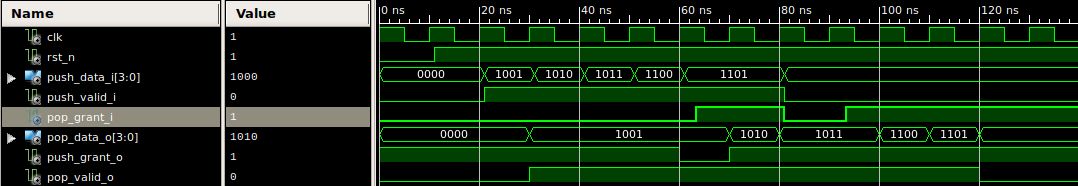
\includegraphics[width=15cm]{images/fifo-simulation}
\caption{\label{fig: FIFO simulation} \fifo's simulation.}
\end{figure}

\subsubsection{\paritycheck}
\label{subsubsection: Parity Check}

Data that it is \textit{pushed} by the sender includes a parity bit. Therefore, the task of this block is to calculate the parity of the raw data (without the parity bit) and check if they match. This module can be divided in three \textit{concurrent} blocks. The first one is to retrieve the parity bit, which can be in the MSB or LSB. This will depend on constant values defined on "my\_pkg.vhd". The second one, calculates the parity of the raw data (without the included parity bit) by XOR-ing all its bits. If the result is 1, the calculated parity will be \textit{odd} and \textit{even} if 0. The third one compares if the included parity and the calculated one match. If they do, \textit{valid\_o} will be 1 and 0 if they do not. As this is a concurrent design, there is an enable condition that has to be true, which happens when the receiver is ready to read new data (grant\_i) and the \fifo has data available (valid\_i).  Its output (valid\_o) will be 0 if this condition is not met.

The testbench checks the correct operation of the logic, taking into account that the parity in the data will be in the LSB and will be ODD.  This means that the LSB will be 1 if the parity is ODD or 0 if it is EVEN. This parameters can be easily changed in "my\_pkg.vhd".  

\begin{figure}[ht]
\centering
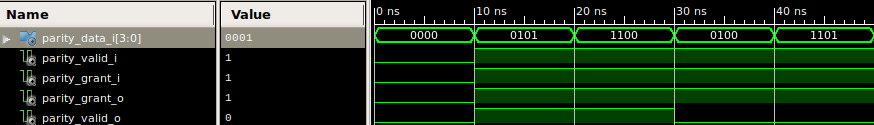
\includegraphics[width=15cm]{images/parity-check-simulation}
\caption{\label{fig: ParityCheck simulation} \paritycheck's simulation.}
\end{figure}

Four different cases are shown in Figure \ref{fig: ParityCheck simulation}.
\begin{itemize}
	\item data\_i=0101: The raw data is 010.  Therefore, it has ODD parity which matches the included one so valid\_o is 1.
	\item data\_i=1100: The raw data is 110.  Therefore, it has EVEN parity which matches the included one so valid\_o is 1.
	\item data\_i=0100: The raw data is 010.  Therefore, it has ODD parity which does not match with the included one so valid\_o is 0.
	\item data\_i=1101: The raw data is 110.  Therefore, it has EVEN parity which does not match the included one so valid\_o is 0.
\end{itemize}

\subsubsection{FifoParityCheckerUB\_TOP}
\label{subsubsection:FifoParityCheck TOP}
The modules described in section \ref{subsubsection: Fifo} and \ref{subsubsection: Parity Check} are instantiated in this one.  Its testbench also mimics the signals in the example, the same way as described in section \ref{subsubsection: Fifo}.  The only difference is that now valid\_o will be different due to the ParityCheck module described in section \ref{subsubsection: Parity Check}.  The simulation is shown in Figure \ref{fig: FIFO and Parity TOP simulation}.

\begin{figure}[ht]
\centering
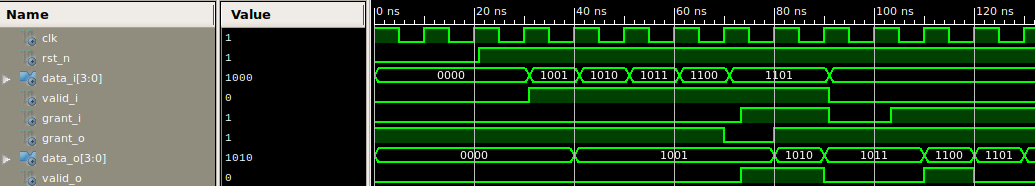
\includegraphics[width=15cm]{images/fifo-paritycheck-TOP-simulation}
\caption{\label{fig: FIFO and Parity TOP simulation}\fifo and \paritycheck TOP module's simulation.}
\end{figure}

\subsection{Test Environment}
This module serves as a testbench for the one described in section \ref{subsubsection:FifoParityCheck TOP}.  The FifoParityCheckerUB\_TOP module is instantiated in the TestEnvironment\_TOP module as well as the three ones described next.

\subsubsection{Traffic Generator}
\label{subsubsection:Traffic Generator}
This module receives the \textit{test vectors} provided by the stimulus in the testbench. It separates the raw data and the traffic type (Table \ref{table:traffic type}) to be sent to their respective modules. Depending on the traffic type and whether the \fifo is full or not (grant\_o), \textit{valid\_i} changes its state depending on the current test vector.  The structure of the test vector is: N bits of data and 2 bits for the traffic type.  The array with the test vectors can be changed in "my\_pkg.vhd".

\begin{figure}[ht]
\centering
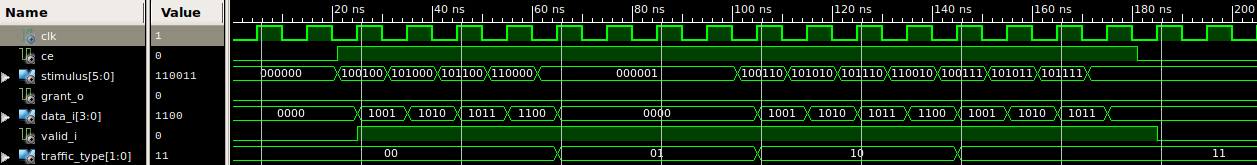
\includegraphics[width=15cm]{images/traffic-generator-simulation}
\caption{\label{fig:Traffic Generator Simulation}Traffic Generator module's simulation.}
\end{figure}

The result of the simulation is shown in Figure \ref{fig:Traffic Generator Simulation}, where it can be seen how data\_i and traffic\_type change accordingly to stimulus.

\subsubsection{Grant\_in Generator}
As the name indicates, this module generates the state of grant\_i. It takes a two bit vector with the traffic type as input and changes its output (\textit{grant\_i}) accordingly.  This module can be seen as a 2-to-4 decoder with a ''special feature'' for the ''11'' input, which is a frequency divider (by 2).  The four different possibilities that traffic\_type represents are described in table \ref{table:traffic type}.

\begin{table}
\centering
\caption{Traffic Type}
\label{table:traffic type}
\begin{tabular}{|c|c|c|c|}
\hline
Traffic Type & Status   & grant\_i & Function                                                                    \\ \hline
00           & FULL     & 0        & Data is pushed unti the \fifo is full and nothing is poped. \\ \hline
01           & EMPTY    & 1        & Data is constantly poped but not pushed.                          \\ \hline
10           & 100\% BW & 1        & Data is pushed and poped simultaneously.                                    \\ \hline
11           & 50\% BW  & Changes  & Data is poped 50\% of the time that it is pushed (50\% BW).                                                   \\ \hline
\end{tabular}
\end{table}

The simulation shown on Figure \ref{fig:Grant_In Generator Simulation} matches with table \ref{table:traffic type}.

\begin{figure}[ht]
\centering
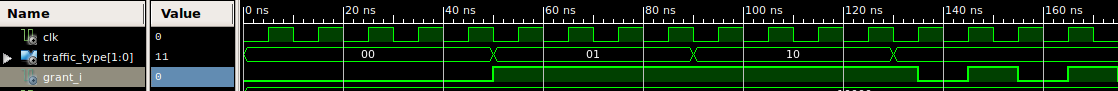
\includegraphics[width=15cm]{images/grant-in-generator-simulation}
\caption{\label{fig:Grant_In Generator Simulation}Grant\_In Generator module's simulation.}
\end{figure}

\subsubsection{Checker}
This module checks the incoming and outcoming data.  It counts poped data with correct parity (pass) and incorrect parity (drop), which depends on the output of the \paritycheck module described in Section \ref{subsubsection: Parity Check}.  It also checks if there is data loss.  The ''Checker'' module is then divided into two separate \textit{concurrent} blocks shown in Figure \ref{fig:Checker diagram}.  It is also important to note that it contains a chip enable input (''ce'') that has to be set to 1 when the test starts (test vectors are being looped) and set to 0 when finished.

Pass and drop are chosen to be 8-bit output ports.  Therefore, the length of the test (number of test vectors) has equal or less than 255, otherwise these two ports might overflow.  In case there is need for larger tests, these ports can have more bits, but the module will have to be re-synthesized.  These two counts are done concurrently in the ''Pass and Drop'' block of the module.  They are obtained by checking whether valid\_o is 1 (pass) or 0 (drop).  There is a condition for this, which is that grant\_i has to be 1.  This means that the receiver is ready to pop new data and data\_o is updated.

As the design is based on a \fifo, the N-poped value will be the N-pushed one.  Therefore, the ''loss block'' checks if the N-poped data matches the N-pushed one.  All data that it is pushed into the \fifo is stored into the RAM.  A 4-bit counter keeps track of how many pushes have been and its output is used as an address pointer.  Another 4-bit counter keep track of how many pops have been and its output is used as a read pointer.  Whenever data is poped, the corresponding RAM position is read to obtain the N-pushed value and it is compared with data\_o which corresponds to the N-poped value.  They are compared in a simple comparator that sets its output to 1 if both its inputs are equal.  This signal acts as the chip enable for the third 4-bit counter which is where the number of lost data is counted.

\begin{figure}[ht]
\centering
\includegraphics[width=15cm]{images/checker_diagram}
\caption{\label{fig:Checker diagram}Checker module's block diagram.}
\end{figure}

The testbench was done so as to mimic the example of the exercise.  As there is no lost data there, a data\_o value was changed to test the ''loss block'' operation.  Therefore, 3 passed, 2 dropped and 1 lost values are expected and the simulation displayed in figure \ref{fig:Checker simulation} shows the correct operation of this module.

\begin{figure}[ht]
\centering
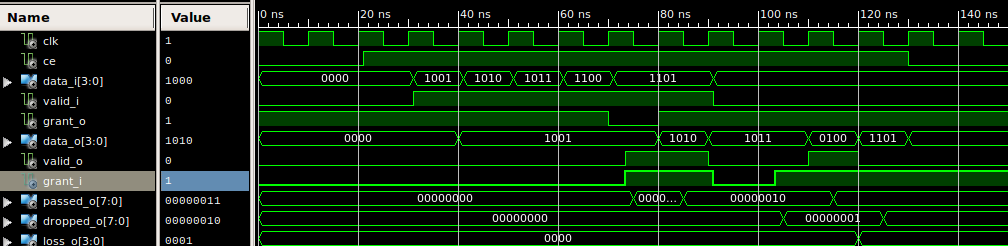
\includegraphics[width=15cm]{images/checker-simulation}
\caption{\label{fig:Checker simulation}Checker module's simulation.}
\end{figure}

\subsubsection{TestEnvironment\_TOP}
All the modules described before are instantiated and connected accordingly as requested in the exercise.  The testbench was designed to test the different type of traffic requested:

\begin{enumerate}
	\item Full the \fifo.
	\item Empty the \fifo.
	\item Random traffic, at max BW (this means that pop\_grant\_i is always 1).
	\item Random traffic, with random pop\_grant\_i (50\% low, 50\% high).
\end{enumerate}

An array with 16 test vectors was used in the testbench for this module.  They have the same structure as described in Section \ref{subsubsection:Traffic Generator}.  There are 4 of them for each type of traffic as the \fifo was tested with a depth of 2 (or 4 slots).  The result obtained in the simulation is displays on Figure \ref{fig: TestEnvironment simulation}.

\begin{figure}[ht]
\centering
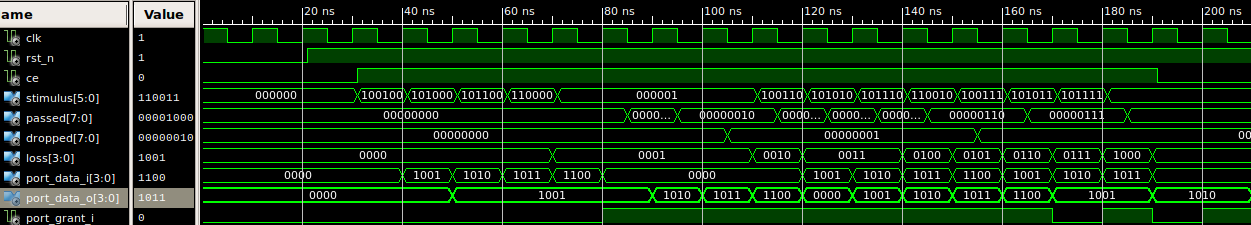
\includegraphics[width=15cm]{images/testenvironment-simulation}
\caption{\label{fig: TestEnvironment simulation}TestEnvironment module's simulation.}
\end{figure}

\section{Conclusion}
Each section and subsection showed the implemented design and their corresponding testbench.  A layer-design allowed to code and test all the modules needed in an efficient manner.  By testing simpler modules individually to guarantee their correct operation made it easier to instantiate them in their TOP design.  This also allowed testing the TOP designs to be easier.

\end{document}
